\subsection{Experiência 3}

Esta experiência possibilitou o entendimento do sistema de DNS bem como a configuração de NAT num router comercial.

\begin{figure}[!h]
\centering
  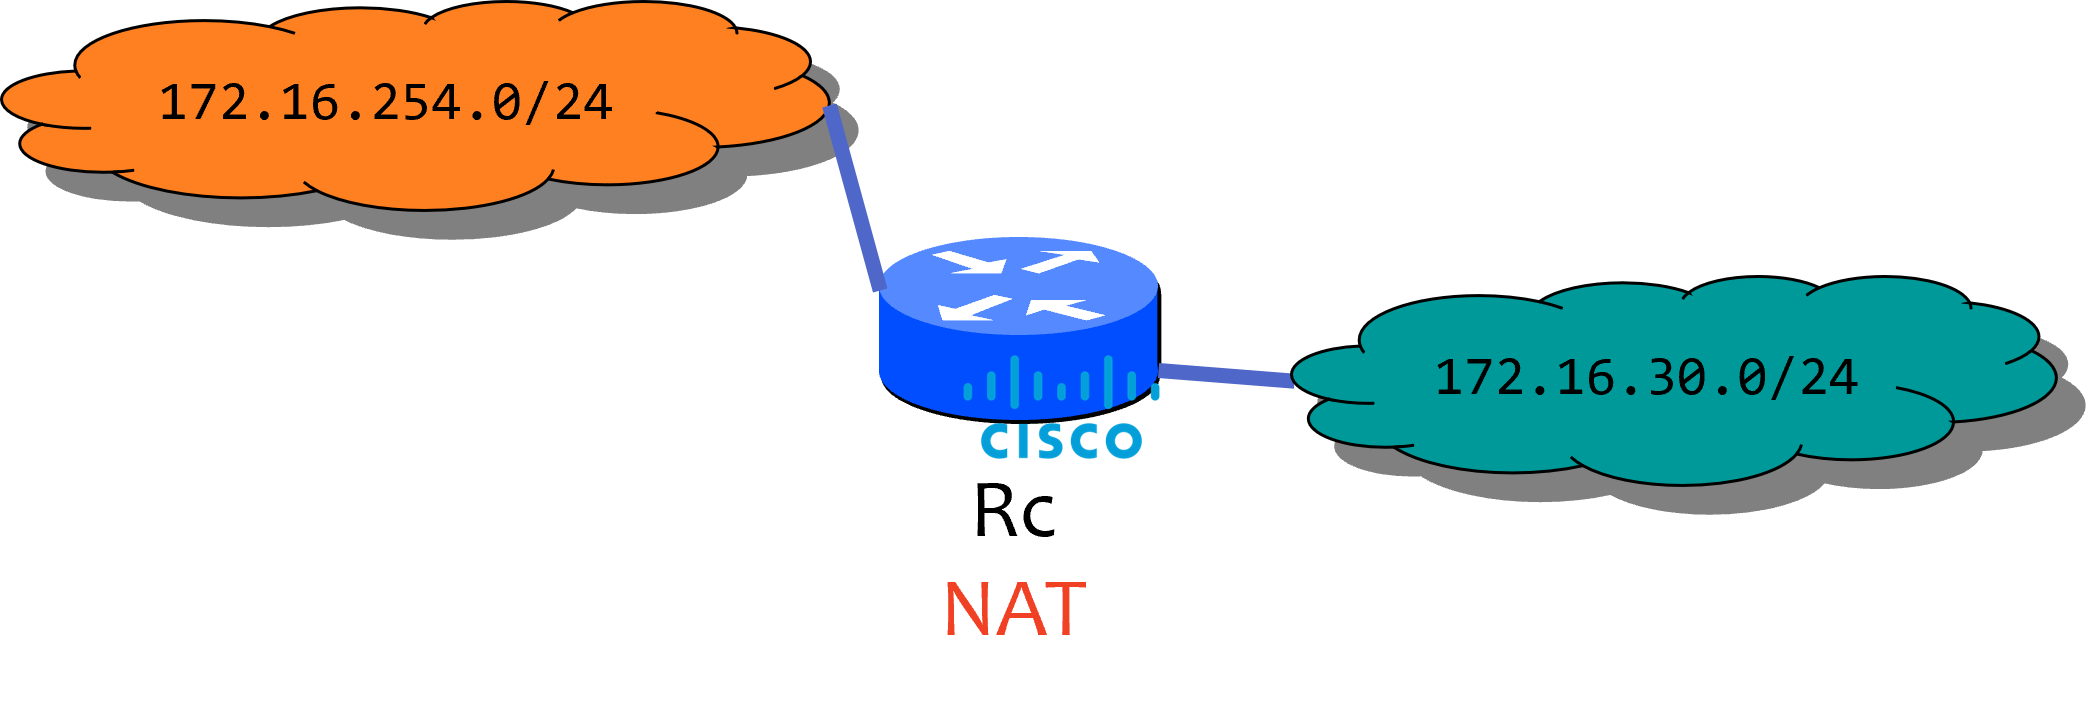
\includegraphics[width=.4\linewidth]{img/net-routing-nat-cisco.png}
  \caption{Estrutura da rede}
\end{figure}

\subsubsection{Questões}

\paragraph{Como configurar uma rota estática num router comercial?}

Executando o seguinte comando:  
    \begin{center} \lstinline{ip route 172.16.40.0 255.255.255.0 172.16.30.2} \end{center}

O primeiro endereço refere-se ao prefixo de origem dos pacotes, o segundo endereço é a máscara de sub-rede, e o último endereço é o gateway dos pacotes.

\paragraph{Como configurar NAT num router comercial?}
Para configurar a NAT deve-se seguir os seguintes comandos:
 - Identificar a interface de rede com o comando: interface FastEthernet0/0
 - Atribuir o endereço de IP que a interface vai tomar nessa NAT com: ip address 172.16.30.1 255.255.255.0
 - Especificar o tipo de NAT interno ou externo (neste caso externo): ip nat inside

Após configurar a interface deve configurar-se a pool de endereços exteriores disponiveis com: ip nat pool ovrld 172.16.254.45 172.16.254.45 prefix-length 24

Por fim, basta configurar a pool IP's internos:
\begin{itemize}
    \item ip nat inside source list 1 pool ovrld overload
    \item access-list 1 permit 172.16.40.0 0.0.0.7
    \item access-list 1 permit 172.16.30.0 0.0.0.7
\end{itemize}


\paragraph{O que faz a NAT?}
NAT é uma técnica que permite mapear uma gama de endereços IP para outra gama de endereços IP mudando o IP dos pacotes enviados enquanto estão em trânsito. É utilizada geralmente para mapear o endereço IP público fornecido por um ISP para o endereço privado da máquina do utilizador.

\paragraph{Como configurar o serviço de DNS no host?}
Pode-se configurar traduções especificas em /etc/hosts como fizemos com o mapeamento do endereço de youtubas. Pode-se configurar um servidor central que faz a tradução no ficheiro /etc/resolv.conf adicionando: nameserver {IP_DNS}

\paragraph{Que pacotes são trocados pelo DNS e que informação é transportada}
São observados dois tipos de pacote muito semelhantes. Ambos transportam o hostname sobre o qual se quer saber o IP. A resposta aos pacotes do tipo 'A' é um endereço IPv4, já a resposta ao pacotes AAAA é um endereço IPv6.

\paragraph{Que pacotes ICMP são observados e porquê?}
O traceroute tenta encontrar o número mínimo de saltos para alcançar um determinado destino. Para isso gera pacotes UDP com TTL crescente partindo de 1. Quando recebe um pacote ICPM que informa que TTL foi excedido o traceroute sabe que necessita de pelo menos mais um valor de TTL para alcançar o destino. No nosso caso como o destino não aceita pedidos é ainda enviado um pacote ICPM que informa que a porta é inalcançável.

\paragraph{Quais são os endereços IP e MAC associados a pacotes ICMP e porquê?}
Os endereços IP de destino são sempre da nossa máquina, os de origem correspondem aos vários IP intermédios pelos quais os pacotes devem viajar até alcançar o destino (Figure 18). Cada vez que o traceroute aumenta o TTL, o endereço de origem muda, o que significa que o pacote atingiu mais um nó. O endereço MAC de origem é sempre o endereço MAC da interface virtual do computador host, o o endereço de destino é o MAC da interface virtual do Guest OS.

\paragraph{Quais são as rotas na sua máquina? Qual o seu significado?}
A rota com origem em 0.0.0.0 e  destino em 172.24.64.1 é a default gateway é indica por onde devem ser enviados os pacotes caso não possam ser encaminhados para a rede local. (Figure 19)

A rota com origem em 172.24.64.0 e gateway 0.0.0.0 é a rota inválida para pacotes com destino inválido.